\chapter{Methods}
\label{chapter:methods}

The research followed design science methodology which was then complimented with semi-structured thematic interviews, participatory methods and Lean Service Creation tools. This chapter introduces the methodologies and tools used and application of them in the study.

\section{Overview of Methods}
\label{section:overview}

\subsection{Design Science Research Methodology}

Design research is a research method which aims to change the world by making it better \parencite{Johannesson:2014}. In addition \textcite{Aken:2014} describes \emph{Design Science Research DSR} to be a problem solving research strategy which should produce actionable knowledge in order to address types of field problems. The knowledge is used as a means, not as an end which means that the knowledge can be applied in a direct way to realize the desired outcomes. This is done by developing artefacts which should solve the problem experienced by people \parencite{Johannesson:2014}.

According to \textcite{Johannesson:2014} the designed artefact can be a construct, method, model or instantiation. Constructs help to formulate problems and answers for them meaning that they are definitional knowledge. Definitional knowledge means that with them it is possible to speak statements about the world rather than make the statements about the world. Methods define guidelines and processes which are meant to solve problems and achieve goals. Additionally, methods can be informal and be used as best practices. Models are used to represent possible solutions for a practical problem which means that they can be used to define the construction of the artefact. Lastly, instantiations are systems which are used in practice.

As stated above, the design science research is driven by the field problems rather than knowledge problems, meaning that the problem is defined in the real world situation by stakeholders. 

The design science research aims to produce a solution concept which would then be used to solve the field problem. This solution concept is used in the context by a design proposition. Design proposition can be formulated using CIMO-logic, which stands for this problem-in-\emph{C}ontext it is useful to use this \emph{I}ntervention to produce through these \emph{M}echanisms this \emph{O}utcomes.

DSR-project has three parts \begin{enumerate}
\item An explanatory part which consist of analyzing and framing of the chosen type of field problem.
\item A design part when an intervention is designed and tested in an iterative way.
\item A testing part where the final version of the intervention is tested. \parencite{Aken:2014}
\end{enumerate}

\textcite{Peffers:2007} created a methodological framework for doing design science which complements and gives more precise activities for doing a DSR-project. This methodological framework is illustrated in the Figure~\ref{fig:dsrm-model}. The first activity is \emph{problem identification and motivation} where the specific research problem and justification of the value of a solution is defined. \emph{Defining the objectives for a solution} is the second activity where the objectives of a solution are inferred from the problem definition.

\begin{figure}[ht]
  \begin{center}
    % here the width of the figure is set to 9 cm
    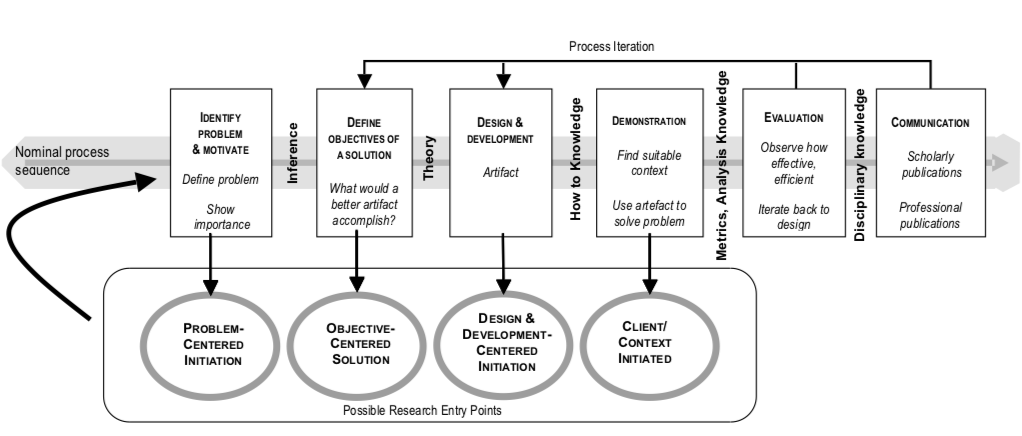
\includegraphics[width=0.80\textwidth]{dippa/images/DSRM-model.png}
    \caption{Eeyore, or Ihaa, a very sad donkey.}
    \label{fig:dsrm-model}
  \end{center}
\end{figure}

Next, the artifact which can be model, method, instantiation or construct is \emph{designed and developed}. Then the artifact is used to \emph{demonstrate} how it can be used to solve the identified problem. The artifact is \emph{evaluated} on how well it supports solving the research problem. This is done by comparing the objectives of a solution to the actual observed and measured results from the demonstration. Finally, the knowledge should be communicated to researchers.

\subsection{Semi-structured Thematic Interview}

According to \textcite{Wilson:2013} a semi-structured interview combines open-ended exploration with predefined questions and it usually follows a interview guide which offers a frame to conduct such interviews. The interview guide consists of an introduction to the topic and the purpose of the interview, a list of topics and predefined questions to ask, probs and promts and comments to end the interview.

A Semi-structured interviews are done in a conversational manner even though there can be predetermined questions. It is a good method in order to investigate behaviours, opinions and emotions as well as to gather experiences. It provides a way to get more details about a topic where there is already some knowledge, but it lacks a deeper understanding. For the interviewee the semi-structured interview allows to focus on topics which they feel more important. In addition compared to the structured interview, the answers are open and not yes or no type of answers. \parencite{Cliffod:2010,Wilson:2013}

According to \textcite{HH:2001} semi-structured thematic interview is based on the focused interview which was published in a book \emph{The Focused Interview} written by Merton, Fiske and Kendall. and it provides a framework for the discussion. The most relevant aspect of thematic interview is that the interview is going forward based on the themes rather than detailed questions. This allows the interviewees to answer more freely with their own wordings in order to bring their experiences to the center of attention and thus for the interviewer it is possible to collect insights about what people do and think \parencite{Cliffod:2010}.

As stated above, semi-structured interview as well as thematic interview have many strengths considering the flexibility, gathering experiences and the comparison between the interviews. However, it is important to be aware of that the interviewer do not put words into the interviewee's mouth or guide the discussion into particular answer during the interview. Since, the semi-structured interview is flexible, it is crucial for the interviewer to be aslo consistent in order to make comparisons between the interviews. \parencite{Wilson:2013}

\subsection{Lean Service Creation}

\emph{Lean Service Creation LSC} is in practice a set of tools which help multidisciplinary teams to create new services and products. It is based on Lean Startup, Agile methods and Design thinking. LSC offers canvases which outline the relevant phases in a service creation process and it is at the hands of the user to decide in which order the canvases should be used.

The creators of LSC emphasize the mindset and practices that allow the successful creation of services by these principles:
\begin{itemize}
	% You can use this command to set the items in the list closer to each other
	% (ITEM SEParation, the vertical space between the list items) 
	\setlength{\itemsep}{2pt}
	\item All for team, the team for all.
	\item Love the problem, not the solution.
	\item No matter what you do, be transparent about it.
	\item Never stop iterating, never stop learning.
	\item See the forest, see the trees, spot the squirrel
\end{itemize} \parencite{LSC}

\section{Research Implementation}
\label{section:research-implementation}

Design science aims to create things to serve human purposes. The four types of products that design science aims to produce are constructs, models, methods and implementations. Design scientists develop ways to perform goal-directed activities which are innovative and valuable. \parencite{Salvatore:1995} Since, the purpose of this study is to design a method to sell services for private housing companies it is justified to use design science. Next chapters describes how the actual research was done.

\subsection{Activity 1: Problem Identification and Motivation}

Based on the DSRM process the study started with the first activity, problem identification and motivation. The case company was in the situation where they needed to expand their sales, and in order to grow bigger in Finland, they needed limited liability housing companies as clients. The problem in acquiring them as clients was that the case company had not done business to customer selling much and they needed to gain more understanding about how the limited liability housing company works and makes decisions. This problem then lead to the first research question \emph{What affects the buying decision making in a limited liability housing companies}.

In addition to understanding the decision making in limited liability housing companies, it was important to discover a sales process which would take into account the case company's and partners viewpoints as well as the end-customers' viewpoints in order to make acquiring limited liability housing companies as clients easier, faster and unified. From this problem the second research question was formed as \emph{What kind of sales process is proper for selling services for limited liability housing companies?}

Literature review was conducted in the Chapter 2 and it included  the research about limited liability housing company and experience mapping. Limited liability housing companies were studied in order to understand the operation and the legal backgrounds of its actions. The research about customer journey mapping was done to find out the benefits and the usage of it in order to design a sales process that would be in a form of a customer journey.

In order to understand the motivation and the problems of energy companies, the researcher participated in several partner meetings and observed them. In addition the researcher did observation at the workplace and that knowledge was applied in several occasions. The researcher also used few canvases from the LSC in order to make communication easier with the relevant stakeholders and to make the discussed topics more tangible.

\subsection{Activity 2: Defining Objectives for a Solution}
What artefact can be a solution and which requirements are important for stakeholders?

The second activity of a DSRM, defining objectives for a solution was done by interviewing the board members of limited liability housing companies. Since, the purpose of first research question was to find out what affects the purchasing decision making in the housing board it was justified to conduct semi-structured thematic interviews in order to discover the real feelings and operations inside the board. The interview was chosen because it provides a way to get deeper understanding by collecting detailed information \parencite{Johannesson:2014}. In addition the semi-structured interview allows the discussion to flow freely and the interviewees were able to describe the situations more broadly compared to structured interview.

The interviews were done with people who were currently in a housing board. To gain broader understanding the researcher did interviews with people of different age and experience level in the board. The researcher conducted 6 interviews that lasted from 40 to 80 minutes. The interviews were performed face to face meetings and recorded in order to listen and analyze them afterwards. The semi-structured thematic interview was divided into four main themes in order to answer the RQ1: \emph{What affects the buying decision making in a private housing company board}. These themes were defined in order to gain insights about why people go to board, how the board  operates in practice and what is affecting their work. 

The themes covered in the interviews were as follow: working in a board of housing company, decision making in the board, influences on housing company operations and energy efficiency.  The first theme dealt with reasons why the interviewees were working in the board and their feelings about the work in general.  Second theme covered the process of decision making with examples of previously made investment decisions and the role of money in them.  Third theme concentrated to learn about influences which affects the operations of the board as well as who the board trust and where they find information related to services provided for private housing companies.  Lastly the energy efficiency topic discovered how well is energy efficiency topics understood in the boards of the housing companies and the relevance of it.

Analyzing of the interviews was done by listening the interviews again and taking notes of relevant points and afterwards clustering them into categories. The researcher divided the notes based on the LSC user insight canvas for user needs and problems, what surprised the researcher and what the user thinks and feels. According to \textcite{HH:2001} the researcher knows the interview material so well that it is easy for her to recognize the themes covered and make notes about dialogue when needed. Thus, in this study the researcher did not transcribe the interviews since there were only 6 interviews to be analyzed and the researched conducted the interviews alone. With the use of LSC canvas for analyzing the interviews the design decisions and objectives for a solution were defined from the user's perspective.

In addition to the interviews, the researcher participated many meetings where the energy company was present. From the meetings, the researcher gained understanding on how well do the energy companies understand the limited liability housing companies as their customers and how much they have communication with them. Additionally, the researcher learned about the drivers to have case company's solution as one of the company's service offering. To understand more about the energy company the researcher and the team divided energy companies into categories describing the team, will and speed in order to provide the solution into  their needs.

Regarding the second research question the researcher and team filled a customer engagement canvas together with one energy company. Customer engagement canvas was chosen from Lean Service Creation because it was familiar for the researcher and the team. Moreover, the canvas helps to list all the steps from rising customer awareness, engagement, purchase, use, use more and advocate combined with the touchpoints. By listing also the enablers and problems it was easier to discover problems and the case company also gained insight about their work. 

For this study, the researcher limited the focus on type of energy companies who are interested and motivated to have new service offering for limited liability housing company but do not have enough resources to proceed with the topic. For this specific type of energy company, the team decided to compose a sales process guidance on how to get limited liability housing companies as clients of their new service provided by the case company. To design this kind of guidance it was decided to use customer journey creation to support the design. With the help of guidance it should be possible to increase sales, reduce lead times and lower the customer acquisition costs.

\subsection{Activity 3: Design and Develop}
Create artefact which addresses the problem and fulfills requirements

The second activity in design science research is design and develop and its purpose is to design an artefact which addresses the stated problem and fulfills the defined objectives \parencite{Johannesson:2014}. So, to answer the second research question \emph{What kind of sales process could help engaging limited liability housing companies as clients?} it was decided to compose a guidance with the help of customer journeys which would could be used inside the case company as well as the energy companies. As stated in the Chapter 3 the customer journey is a good tool to XXX because XXX.

To design a better way and guidance on how to acquire customers it was first necessary to go through the current customer journey. For this, the researcher used LSC canvas for visualizing customer engagement. The canvas was filled with one energy company and it was also complemented with the knowledge gained from other meetings with energy companies. From this work it was decided to focus on the first three steps in customer engagement canvas which were awareness, engagement and purchase because it was identified that those are the biggest bottlenecks. Additionally the case company's product is sold by the partners and they can sell the service in which form the want but they lack the knowledge about how to actually approach the limited liability housing companies.

For creating the guidance the researcher and the team designed three different fake ads which were all looking the same but the pricing model was different in each of the ads in order to find out which model the limited liability housing boards would choose and why. In addition the researcher and the team designed personalized offers for the limited liability housing companies in order to rise the engagement and with the limited liability housing company.

From the interviews done with the limited liability housing companies, it was clear that in the guidance the clear communication, making things as simple as possible and providing support are important when being in contact with them. With this in mind the the researcher participated one open day organized by an energy company in Finland. There the researcher was able to provide support and answer the questions about the service.

\subsection{Activity 4: Demonstrate}
\subsubsection*{Limited Liability Housing Company Fair}
The three different fake ads designed were tested in the limited liability housing company fair which was aimed for the board members of limited liability housing companies. The specific fair was chosen because the main audience there were purely the board members because the idea behind the fair is to present services and products for limited liability housing companies. The fake ad testing was done together with one energy company who is case company's partner. This was done because the partner company had a ready service which was already in the market but they were struggling with the pricing model.

So, the fake ads had three different kinds of pricing models to cover the provided service which were as follows:
\begin{itemize}
	% You can use this command to set the items in the list closer to each other
	% (ITEM SEParation, the vertical space between the list items) 
	\setlength{\itemsep}{2pt}
	\item Investment plus a monthly service fee,
	\item A monthly service fee.
	\item A monthly service fee which is covered by the saved energy fees.
\end{itemize}

The ads were shown for 12 people and asked to read and comment the ads. The testing was done mainly in pairs which allowed the other to present the ads and the other to make notes about the test session. The team approach people in the fair and asked if they would be willing to give opinions about the ads. The ads were given for the volunteers and after a moment the people needed to choose one of the ads which had the pricing model that they prefer the most. The team asked reasons behind the choice and also feedback about the ads in order to find out improvement ideas.

\subsubsection*{Energy Company's Open Day}

The researcher participated an open day organized by an energy company in Finland. The purpose was to be there in person and to promote their service which is built on the case company's technology. In the open day the researcher had personalized offers for the area's limited liability housing companies.

The offers all had the same monthly cost but in the offer it was also stated how much is the predicted saving if they would have the service in use. The researcher was able to contact the members of limited liability housing companies in person, answer the questions immediately and also to collect contact information from interested buyers.

The researcher was able to discuss with three members of limited liability housing company. All of them received an offer and their contact information was collected for the energy company to be in contact with them afterwards.

\subsection{Activity 5: Evaluate and Iterate}

In the second to last activity of DSRM the designed artefact is evaluated to see how well it solve the initial problem and fulfil the set requirements. To answer the RQ1 the researcher analyzed the interviews and formed requirements which were then used to form guidance of how the sales process should go.

To answer the RQ2, the researcher together with team did different test to gain insights about what works and what not in acquiring limited liability housing companies as clients. The test were evaluated also from the business perspective and objectives.

Since, the purpose of this study was to gain more knowledge about the limited liability housing companies and a possible sales process which would work as a guidance for the case company and also for the partner energy companies the results were also used in purpose to find out future research areas.

Iteration was not possible to do for the whole process because of the research time span. However, the ads were improved after test sessions and the insights gained from the test sessions were always further used in the next sessions as well as daily work. In addition, the researcher describe the future research ares and recommendations of what should be done next.

\subsection{Activity 5: Communicate}

The last activity of the DSRM consist of communicating the results of the study and this is done through this thesis. In addition, the results are presented in the case company and the guidance of the possible sales process is presented for the case company's energy company partners.






 